\subsection{Variable}\label{subsec:variable}
There are J jobs, indexed with $ j = 1,\dots,J $ and I servers, indexed with $ i = 1,\dots,I $.
\begin{itemize}
    \item $ x_{i,j} \in \{0, 1\}$ indicates whether the job $j$ was done on server $i$
    \item $ s_{i,j} $ the rate that the program is loaded at (MB/s)
    \item $ w_{i,j} $ the rate of computation (TFlop/s)
    \item $ r_{i,j} $ the rate that the result's data is sent back (MB/s)
\end{itemize}

\subsection{Constants}\label{subsec:constants}
Server - i
\begin{itemize}
    \item Maximum storage - $ S_i $ (MB)
    \item Maximum computation capacity - $ W_i $ (TFlop/s)
    \item Maximum communication bandwidth - $ R_i $ (MB/s)
\end{itemize}
Job - j
\begin{itemize}
    \item Required storage - $ s_j $ (MB)
    \item Required computation capacity - $ w_j $ (TFlop)
    \item Required data for results - $ r_j $ (MB)
    \item Utility - $ U_j $ (\$)
    \item Deadline - $ D_j $ (s)
\end{itemize}

\subsection{Optimisation}\label{subsec:optimisation}
\begin{align}
    max \sum_{j=1}^{J} U_j x_{i,j} && \forall i = 1,\dots,I
\end{align}

\subsection{Constraints}\label{subsec:constraints}
Job to server allocation
\begin{align}
    \sum_{i=1}^I x_{i,j} \leq 1 && \forall j = 1,\dots,J \\
    x_{i,j} \in \{0, 1\} && \forall i = 1,\dots,I; j = 1,\dots,J
\end{align}

%% Server resources checking
Server resource available
\begin{align}
    \sum_{j=1}^J s_j x_{i,j} \leq S_i && \forall i = 1,\dots,I
\end{align}
\begin{align}
    \sum_{j=1}^J w_{i,j} x_{i,j} \leq W_i && \forall i = 1,\dots,I
\end{align}
\begin{align}
    \sum_{j=1}^J (r_{i,j} + s_{i,j}) x_{i,j} \leq R_i && \forall i = 1,\dots,I
\end{align}

%% Within deadline
Process completed within deadline
\begin{align}
    \frac{S_j}{s_{i,j}} + \frac{W_j}{w_{i,j}} + \frac{R_j}{r_{ij}} \leq D_j && \forall i = 1,\dots,I; j = 1,\dots,J
\end{align}

Resource usage
\begin{align}
    0 \le s_{i,j} && \forall i = 1,\dots,I; j = 1,\dots,J
\end{align}
\begin{align}
    0 \le w_{i,j} && \forall i = 1,\dots,I; j = 1,\dots,J
\end{align}
\begin{align}
    0 \le r_{i,j} && \forall i = 1,\dots,I; j = 1,\dots,J
\end{align}

\subsection{Problem Case Explanation}\label{subsec:problem-case-explanation}
\begin{itemize}
    \item Equation 1 is the objective function that maximises the sum of the job utility for jobs completed.
    \item Equation 2 and 3 enforce that a job is only done on a single server.
    \item Equations, 4 to 6, ensures that the server resource used are within the maximum resources available.
    \item Equation 7 enforces that the job will be completed within the deadline on only the servers that is a job runs on.
    \item Equations, 8 to 10, ensures that resource speeds are within a valid range of greater than 0
\end{itemize}

\subsection{Example cases}\label{subsec:example-cases}
\begin{figure}[H]
    \begin{subfigure}{0.5\textwidth}
        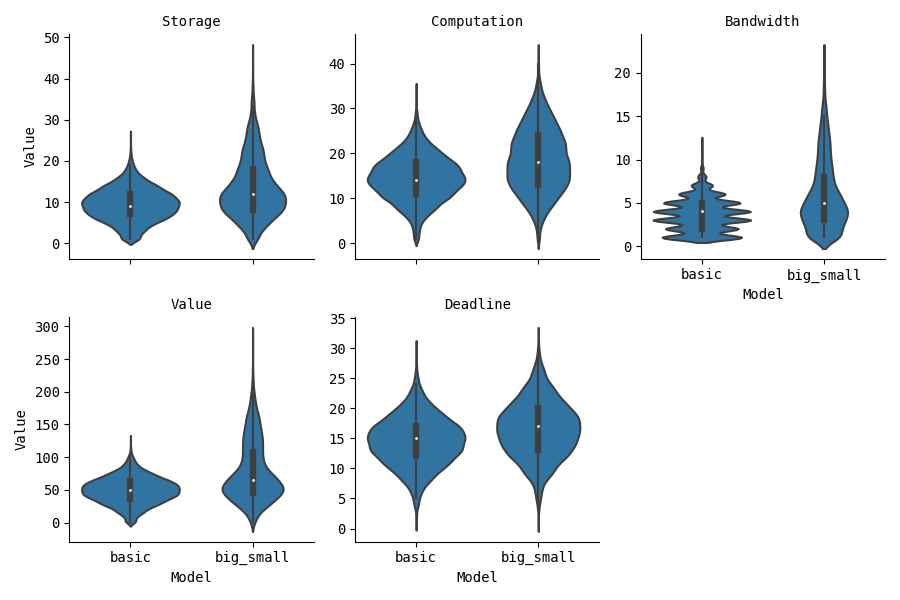
\includegraphics[width=1\linewidth, height=5cm]{/images/job_distribution.png}
        \caption{Example jobs}
    \end{subfigure}
    \begin{subfigure}{0.5\textwidth}
        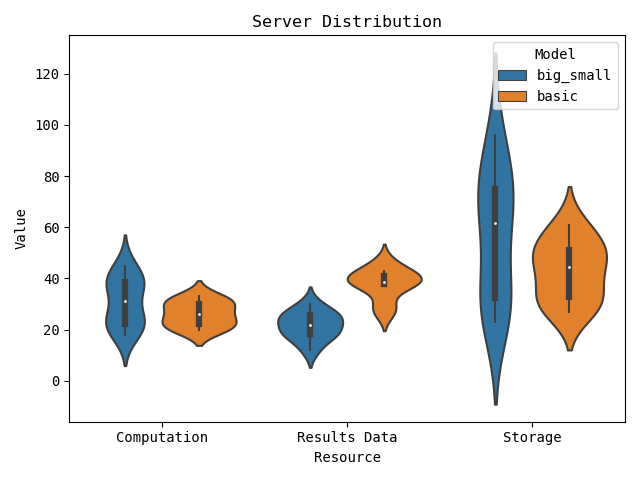
\includegraphics[width=1\linewidth, height=5cm]{/images/server_distribution.png}
        \caption{Example Servers}
    \end{subfigure}

    \caption{Example jobs and servers}
\end{figure}

\subsection{Model creation}\label{subsec:model-creation}
To create each of the jobs and servers we choose a mean and standard deviation for each attribute that is then
used to generate a random number from a normal distribution.
We normalise the value generated to make it an integer and check that the value is greater than zero. \\

\begin{tabu} to 1\textwidth { | X[l] | X[l] | X[l] | X[l] | X[l] | X[l] | }
\hline
Job Attribute & Mean & Std & Server Attribute & Mean & Std \\
\hline
Storage & 10 & 4 & Storage & 45 & 10 \\
\hline
Compute & 15 & 5 & Compute & 30 & 5 \\
\hline
Results data & 5 & 4 & Bandwidth & 40 & 5 \\
\hline
Utility & 50 & 20 & & & \\
\hline
Deadline & 15 & 4 & & & \\
\hline
\end{tabu}